\chapter{Methodology\label{cha:chapter3}}

This section determines the requirements necessary for X. This includes the functional aspects, namely Y and Z, and the non functional aspects such as A and B.
\section{Overview\label{sec:chapter3:overview}}

% In this chapter you will describe the requirements for your component. Try to group the requirements into subsections such as 'technical requirements', 'functional requirements', 'social requirements' or something like this. If your component consist of different partial components you can also group the requirements for the corresponding parts.

% Explain the source of the requirements.

% Example: The requirements for an X have been wide
% ly investigated by Organization Y.

In his paper about Z, Mister X outlines the following requirements for a Component X.

% \input{./chapters/chapter3/overview}
\section{Hysteretic neural networks\label{sec:chapter3:hnn}}
\subsection{Play and Prandtl-Ishlinskii networkds\label{sec:chapter3:play-and-pi-networks}}
\\
Consider $K > 0$ play operators. Each of them maps an initial state $p_{0}^{k} \in \mathbb{R} $ and an input sequence $x_1, x_2, \ldots$ to an output sequence $p_{1}^{k}, p_{2}^{k}, \ldots \ $, i.e.,

% \begin{equation}\label{eqn:input_to_op_output_mapping}
\begin{equation*}
  p_{0}^{k}, (x_1, x_2, \ldots) \mapsto (p_{1}^{k}, p_{2}^{k}, \ldots), k = 1, \ldots, K
\end{equation*}

The $k$th play operator is given by:

\begin{equation}\label{\eqn:chapter3:play-operator}
  p_{n}^{k} = G(x_{n}, p_{n-1}^{k}, w^{k}) := p_{n-1}^{k} + \Phi(w^{k} x_{n} - p_{n-1}^{k}), n = 1, 2, \ldots
\end{equation}

where $w^{k}$ are parameters and

\begin{equation}\label{\eqn:chapter3:phi}
  \begin{aligned*}
    \Phi(x) =
    \begin{cases}
      x - \frac{1}{2}, & x > \frac{1}{2} \\
      0,               & -\frac{1}{2} <= x <= \frac{1}{2} \\
      x + \frac{1}{2}, & x < \frac{1}{2}
    \end{cases}
  \end{aligned*}
\end{equation}

See Fig. \ref{fig:chapter3:phi}

\begin{figure}[htb]
  \centering
  \resizebox{8cm}{!}{\documentclass{standalone}
\usepackage{tikz}
\begin{document}
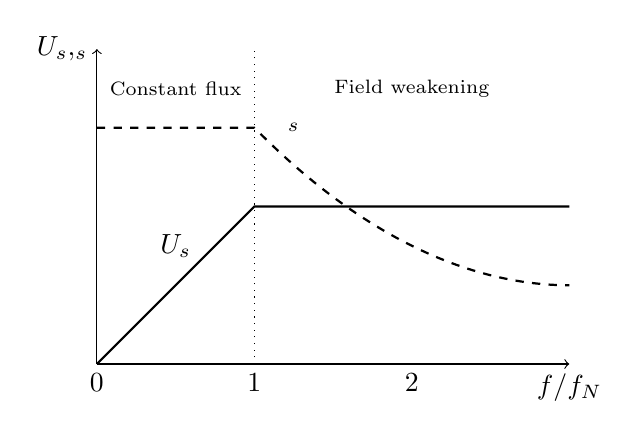
\begin{tikzpicture}
% horizontal axis
\draw[->] (0,0) -- (6,0) node[anchor=north] {$f/f_N$};
% labels
\draw	(0,0) node[anchor=north] {0}
		(2,0) node[anchor=north] {1}
		(4,0) node[anchor=north] {2};
% ranges
\draw	(1,3.5) node{{\scriptsize Constant flux}}
		(4,3.5) node{{\scriptsize Field weakening}};

% vertical axis
\draw[->] (0,0) -- (0,4) node[anchor=east] {$U_s,\varPsi_s$};
% nominal speed
\draw[dotted] (2,0) -- (2,4);

% Us
\draw[thick] (0,0) -- (2,2) -- (6,2);
\draw (1,1.5) node {$U_s$}; %label

% Psis
\draw[thick,dashed] (0,3) -- (2,3) parabola[bend at end] (6,1);
\draw (2.5,3) node {$\varPsi_s$}; %label

\end{tikzpicture}
\end{document}
}
  \caption{$\Phi(x)$}\label{fig:chapter3:phi}
\end{figure}

It can be represented as a recurrent neural network, see Fig. \ref{fig:chapter3:phi}. Note that in such a form the network is not feed-forward.
One can unfold it to make it feed-forwaard, see Fig. \ref{fig:chapater3:play-operator}

\theoremstyle{definition}
\begin{definition}
We call this network a \textsl{play network}. If there are \textsl{m} elements in the sequence ${x_n}$, we say the unfolded network is \textsl{m-unfolded}
\end{definition}

For example, the network in Fig. \ref{fig:chapter3:unfolded-nn} is 2-unfolded.

\subsection{Play layers and Prandtl-Ishlinskii networkds\label{sec:chapter3:play-layers-and-pi-networks}}

\subsection{Training a PI network\label{sec:chapter3:training-pi-network}}
Assume we are given an input sequence $x_1, x_2, \ldots, x_N$ and an output sequence $q_1, q_2, \ldots, q_N$. We perform the following steps in cycle until convergence.

\begin{enumerate}
\item Preparing initial states for the $m$-unfolded network: Fix a vector of initial states $P_0$ and all the weights (denoted by $W$). For each $k=1, \ldots, K$, we calculate recursively $p_{1}^{k}, p_{2}^{k}, \ldots, p_{N}^{k}$ by formula \ref{eqn:chapter3:play-operator}. We denote the corresponding (intermediate) states of the \textbf{PI} operator by
  \begin{equation*}
    P_n = (p_{n}^{1}, \ldots, p_{n}^{K}), n = 1, \ldots, N.
  \end{equation*}
\item Preparing inputs for the $m$-unfolded network: We fix $m$ and group the input sequence into $m$-tuples:
  \begin{equation*}
    \mathbf{x_1} := (x_1, \ldots, x_m), \quad \mathbf{x_2} := (x_2, \ldots, x_{m+1}), \quad \ldots,
  \end{equation*}
  which gives $M := N-m$ tuples $\mathbf{x_1}, \ldots, \mathbf{x_M}$. Next we form a new set of inputs for the $m$-unfolded network, attaching the vectors of intermediate states:
  \begin{equation*}
    \mathbf{y_1} := (P_0, \mathbf{x_1}), \quad \mathbf{y_2} := (P_1, \mathbf{x_2}), \quad \ldots,
  \end{equation*}

\item Training the $m$-unfoled network: We train by stochstic gradient descent the feed-forward $m$-unfolded \textbf{PI} network
  \begin{equation*}
    \mathbb{R}^{K} \times \mathbb{R}^{m} \ni \mathbf{y} \mapsto F_{m}(\mathbf{y}) \in \mathbb{R}^m
  \end{equation*}
  with the inputs $\mathbf{y_1}, \ldots, \mathbf{y_M}$ and the true targets $\mathbf{q_1}, \ldots, \mathbf{q_M}$, where
  \begin{equation*}
    \begin{aligned*}
      \mathbf{q_1} = (q_1, \ldots, \q_m), \quad \mathbf{q_2} = (q_2, \ldots, q_{m+1}), \quad \ldots
    \end{aligned*}
  \end{equation*}

\item We update the initial state $P_0$:
  \begin{equation*}
    P_{0}^{new} := P_{0} - \nabla_{P_0} (F_m(P_0, \mathbf{x_1}) - \mathbf{q_1})^2
  \end{equation*}
\end{enumerate}

\subsection{General hysteretic networks\label{sec:chapter3:general-hysteretic-networks}}
A general network may consist of several play layers (and perhaps standard layers). We can such a network \textsl{hysteretic}, and denote
\begin{equation*}
  p_n = F(X_n, W)
\end{equation*}
where $X_n = (x_1, \ldots, x_n)$ and $w$ is a vector of all weights of the network.

\subsection{Demand/Supply price formation\label{sec:chapter3:demand-supply-price-formation}}
In this model, we assume that the stock exchange accommodates two types of agents, which we call D and N and describe below. We assume that the time takes values $n=0, 1, 2, , \ldots$, and denote the price at time $n$ by $p_n$. By defnition, $p_n$ is the price of last transaction at time $n$. We will see below that demand equals supply at times $n$, but between any two consecutive times $n-1$ and $n$, this need not be the case and there may occur many transactions until demand will have become supply.

\begin{assumption}\label{assumption:chapter3:strategy-of-agentD}
  (Strategy of agents D). Agents D keep track of a trend. They buy stocks iff the price goes up and sell stocks iff the pric goes down. The total amount of stocks that are in possession of all the agents D can be described as a Prandtl-Ishlinksii operator whose input is the price p. We denote this operator by
  $$P_D(p)$$
\end{assuption}
\begin{assumption}\label{assumption:chapter3:strategy-of-agentN}
  (Strategy of agents N). The strategy of each of the agents N is characterized by a non-ideal relay with two fixed threshold $p_1 < p_2$ (different for different agents). The relay is in state 0 if the price higher than $p_2$ and in state 1 if the price is lower than $p_1$. The agent buys one stock whenever his relay switches from 0 to 1 and sells one stock whenever his relay switches frmo 1 to 0. The total amount of stocks that are in possession of all the agents N can be described as a Preisach operator whose input is the price $p$. We denote this operator by
  $$P_N(p)$$
\end{assumption}

The following lemma is direct consequence of the definition of the opeartors $P_D(p)$ and $P_N(p)$.

\begin{lemma}\label{lemma:chapter3:reaction-to-price-change}
  \\
  \begin{enumerate}
    \item If $p$ is increasing, the $P_D(p)$ is increasing (agents D buy) and $P_N(p)$ is descreasing (agents N sell).
    \item If $p$ is descreasing, the $P_D(p)$ is descreasing (agents D sell) and $P_N(p)$ is increasing (agents N buy).
  \end{enumerate}
\end{lemma}

\begin{remark}\label{remark:chapter3:1}
  Since $P_D(p)$ and $P_N(p)$ are not functions but operators, the monotone curves described in \ref{lemma:chapter3:reaction-to-price-change} are not defined only by the current value of $p$, but depend on its prehistory.
\end{remark}

Denote by $B_n$ the total amount of stocks that are in possession of all the agents D and N at time $n$. We will see below in \ref{assumption:chapter3:transitions-between-stabilized-prices}

\begin{assumption}\label{assumption:chapter3:demand/supply-price-formation}
  At each moment $n$, the price $p_n$ is a stable solution of equation
  \begin{equation}\label{eqn:chapter3:demand-supply-price-formation}
    P_D(p_n) + P_N(p_n) = B_n
  \end{equation}
  where the stability notion is explained in Fig.\ref{xxxx}, We will say that $p_n$ is a stabilized price.
\end{assumption}

In order to explain how a stabilized price can change stabilize to the next value, we make the next assumption.

\begin{assumption}\label{assumption:chapter3:transitions-between-stabilized-prices}
  Suppose $p_{n-1}$ is a stabilized price as time $n-1$. In particular, it is a stable solution of equation
  \begin{equation}\label{eqn:chapter3:stable-price-eqn}
    P_D(p_{n-1}) + P_N(p_{n-1}) = B_{n-1}
  \end{equation}
  We assue that between time moments $n-1$ and $n$, some external agents E buy or sell some stocks. As a result, the total amount of stocks that is in possession of agents D and N becomes $B_n$. Moreover, we assume that external agents do not stay at the stock exchange, i.e., the operators (thir densities) $P_D(p)$ and $P_N(p)$ do not chagne in time.
  If $B_n \le B_{n-1}$, then external agents E buy $|B_{n}-B_{n-1}|$ stocks, which increases the price. As as result, agents D also buy. All the stocks bought by agents E and D are sold by agnets N. This leads to the increase of the price to a new value $p_n^1$, where $p_n^1$ is the smallest solution of the equation
  \begin{equation}\label{eqn:chapter3:new-stable-price-eqn}
    P_D(p_n^1) + P_N(p_n^1) = B_n
  \end{equation}
  satisfying the inequality
  \begin{equation}
    p_n^1 \ge p_{n-1}
  \end{equation}

  Note that small values $|B_n - B_{n-1}|$ may correspond to small change of the price as in Fig.\ref{xxxx} or large changes as in Fig.\ref{xxxx}. In the latter case, the price jumps up due to the fold bifurcation.

  If $p_n^1$ is a stable of equation \ref{eqn:chapter3:new-stable-price-eqn}, the, by definition, it coincides with the new stabilized price:
  \begin{equation}\label{eqn:new-price}
    p_n := p_n^1
  \end{equation}
  Otherwise, the price makes several jumps taking semi-stable values $p_n^2, \ldots, p_n^{m-1}$ and a stable value $p_n^m$ (\textbf{hopefully with a finite} m) such that
  \begin{equation}
    missing now
  \end{equation}
  By definition, we set
  \begin{equation}
    p_n := p_n^m
  \end{equation}
  Analogously, the price will leave the stable value $p_{n-1}$ if $B_n > B_{n-1}$. In this case external agents E sell $B_n - B_{n-1}$ stocks, which decreases the price. As a result, agents D also sell. All the stocks sold by agents E and D are bought by agent N.
\end{assumption}

  The last assumption concerns the strategy of external agents E.
  \begin{assumption}
    $B_n$ is a Markov chain. For example, $B_n \sim \mathcal{N}(B_{n-1} + \mu, \tau^{-1})$ with some mean $\mu$ and precision $\tau > 0$
  \end{assumption}

  \begin{remark}\label{remark:chapter3:TODO}
    Set
    \begin{equation}
      G(p) := P_D(p) + P_N(p)
    \end{equation}
  \end{remark}

  Then, formally, the relationship between the price $p_n$ and the noise $B_n$ is the same as Dima's model. \ref{xxx} Though in our second model, there is a number of further restrictions on admissible vlaues of $p_n$ due to Assumption \ref{assumption:chapter3:transitions-between-stabilized-prices}

\subsection{Gradient of networks}\label{sec:chapter3:gradient-networks}
First we only consider \textbf{one play}
\begin{equation}\label{eqn:chapter3:outputs-of-pi-networks}
G(P_{n}, w^{1}) = \sum_{i=1}^{S} \tilde{\theta_{i}} \tanh(\theta_{i} P_{n} + \theta_{i0}) + \tilde{\theta_{0}}
\end{equation}

Where $P_{n} = [p_{1}, p_{2}, \ldots, p_{n}]$, $G(P_{n}, w^{1}) = [y_{1}, y_{2}, \ldots, y_{n}]$, $\forall{i} \in [1, ..., S]$, $\theta_{i} P_{n} = (\theta_{i} p_{1}, \theta_{i} p_{2}, \ldots, \theta_{i} p_{n})$,

So $\tanh(\theta_{i} P_{n} + \theta_{i0}) = [\tanh(\theta_{i} p_{1} + \theta_{i0}), \tanh(\theta_{i} p_{2} + \theta_{i0}), \ldots, \tanh(\theta_{i} p_{n} + \theta_{i0})]$

So $\sum_{i=1}^{S} \tilde{\theta_{i}} \tanh(\theta_{i} P_{n} + \theta_{i0}) + \tilde{\theta_{0}} = [\sum_{i=1}^{S} \tilde{\theta_{i}} \tanh(\theta_{i} p_{1} + \theta_{i0}) + \tilde{\theta_{0}},
\sum_{i=1}^{S} \tilde{\theta_{i}} \tanh(\theta_{i} p_{2} + \theta_{i0}) + \tilde{\theta_{0}},
\ldots,
\sum_{i=1}^{S} \tilde{\theta_{i}} \tanh(\theta_{i} p_{n} + \theta_{i0}) + \tilde{\theta_{0}}] =
[y_{1}, y_{2}, ..., y_{n}]$.

Take $y_{j}$, where $j \in [1, ..., n]$ for example

Let $z_j=\theta_i p_j + \theta_{i0}$ and $f(z_j) = \tanh(\theta_i p_j + \theta_{i0})$, we obtain
\begin{equation}\label{eqn:chapter3:TODO}
y_{j}  &=& \sum_{i=1}^{S} \tilde{\theta_{i}} \tanh(\theta_{i} p_{j} + \theta_{i0}) + \tilde{\theta_{0}}  \\
       &=& \sum_{i=1}^{S} \tilde{\theta_{i}} f(z_j) + \tilde{\theta_{i0}}
\end{equation}

Calculate derivation for $y_{j}$,
\begin{equation}\label{eqn:chapter3:TODO}
\frac{\partial y_{j}}{\partial p_{j}} &=& \sum_{i=1}^{S} \tilde{\theta_{i}} \theta_{i} \frac{\partial f(z_j)}{\partial z_{j}}
\end{equation}

Now let's consider the mapping between $p_{j}$ and $x_{j}$. let $\sigma_{j} = w^{1} x_{j} - p_{j-1}$
\begin{equation}\label{eqn:chapter3:TODO}
p_{j} = \Phi(\sigma_{j}) + p_{j-1}
\end{equation}

and

\begin{equation}\label{eqn:chapter3:TODO}
\Phi(x) =
        \begin{cases}
        x - 1/2, & x > 1/2 \\
        0, & -1/2 < x < -1/2 \\
        x + 1/2, & x < -1/2 \\
        \end{cases}
\end{equation}

Using chain rule, we obtain
\begin{equation}
\frac{\partial y_{j}}{\partial x_{j}} &=& \frac{\partial y_{j}}{\partial p_{j}} \frac{\partial p_{j}}{\partial x_{j}} \\
                                      &=& \sum_{i=1}^{S} \tilde{\theta_{i}} \theta_{i} w^{1} \frac{\partial f(z_j)}{\partial z_{j}} \frac{\partial{\Phi(\sigma_{j})}}{\partial{\sigma_{j}}}
\end{equation}


To consider \textbf{multiple plays} case, we reformulate the derivation as following:

\begin{equation}
\frac{\partial {y_{j}^{1}}}{\partial x_{j}} &=& \frac{\partial{y_{j}^{1}}}{\partial{p_{j}^{1}}} \frac{\partial{ p_{j}}^{1}}{\partial x_{j}} \\
                                      &=& \sum_{i=1}^{S} \tilde{\theta_{i}^{1}} \theta_{i}^{1} w^{1} \frac{\partial f(z_{j}^{1})}{\partial z_{j}^{1}} \frac{\partial{\Phi(\sigma_{j}^{1})}}{\partial{\sigma_{j}^{1}}}
\end{equation}


Now from the architecture, we know that if we have $P$ plays,
\begin{equation}
F = \frac{1}{P} \sum_{k=1}^{P} G^{k}
\end{equation}
Where \(F=[f_1, f_2, ..., f_n]\),
and
\begin{equation}
f_{j} = \frac{1}{P} \sum_{k=1}^{P} y_{j}^{k}
\end{equation}

our derivation is:

\begin{equation}
\frac{\partial f_{j}}{\partial x_{j}} &=& \frac{1}{P} \sum_{k=1}^{P} \frac{\partial {{y_{j}^{k}}}}{\partial {{x_{j}}}} \\
               &=& \frac{1}{P} \sum_{k=1}^{P} \frac{\partial {y_{j}^{k}}}{\partial {p_{j}^{k}}} \frac{\partial {p_{j}^{k}}}{\partial {x_{j}}} \\
               &=& \frac{1}{P} \sum_{k=1}^{P}  \sum_{i=1}^{S} \tilde{\theta_{i}^{k}} \theta_{i}^{k} w^{k} \frac{\partial f(z_{j}^{k})}{\partial z_{j}^{k}} \frac{\partial{\Phi(\sigma_{j}^{k})}}{\partial{\sigma_{j}^{k}}}
\end{equation}

